\documentclass[aspectratio=169]{beamer}
\usepackage{preamble}

\title{Τεχνική αναφορά για NCO‐03‐02}
\subtitle{2η υποχρεωτική εργασία}
\author{Αλέξανδρος Κόρκος}
\institute{Αριστοτέλειο Πανεπιστήμιο Θεσσαλονίκης \\ Τμήμα Πληροφορικής}
\date{\today}

\begin{document}

    \frame{\titlepage}

    \vspace*{\fill}

\begin{center}
    \href{https://creativecommons.org/licenses/by-nc-sa/4.0/deed.el}{
\includegraphics[scale=0.2]{images/cc.png}} \\
    \Rule \\[0.4cm]
    Το έργο αυτό διατίθεται υπό τους όρους της άδειας \textbf{\href{https://creativecommons.org/licenses/by-nc-sa/4.0/deed.el}{Create Commons "Αναφορά Δημιουργού - Μη Εμπορική Χρήση - Παρόμοια Διανομή 4.0 Διεθνές"}}. \\ 
\end{center}



    \begin{frame}{Περιεχόμενα}
        \tableofcontents
    \end{frame}

    \section{Τα όνειρα κοστίζουν}

    \begin{frame}{Social Psychology}
        \lipsum[1]
    \end{frame}

    \begin{frame}
        \begin{figure}
            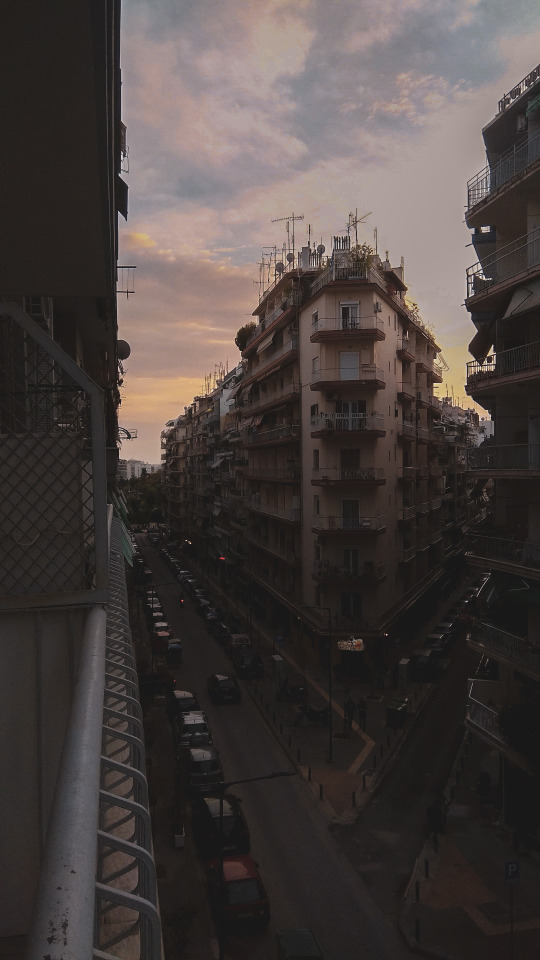
\includegraphics[width=0.25\textwidth]{images/skg.jpg}
            \caption{Θεσσαλονίκη}
            \label{fig:skg}
        \end{figure}
    \end{frame}

    \begin{frame}{Bullet Points}
        \begin{itemize}
            \item Lorem ipsum dolor sit amet, consectetur adipiscing elit
            \item Aliquam blandit faucibus nisi, sit amet dapibus enim tempus eu
            \item Nulla commodo, erat quis gravida posuere, elit lacus lobortis est, quis porttitor odio mauris at libero
            \item Nam cursus est eget velit posuere pellentesque
            \item Vestibulum faucibus velit a augue condimentum quis convallis nulla gravida
        \end{itemize}
    \end{frame}

    \section{Advanced Criminal Law}

    \begin{frame}[fragile]{Code}
        \begin{listing}[H]
            \begin{minted}{python}
            def ypologismos(arithmosTemaxiwn):
                if arithmosTemaxiwn <= 3:
                    return arithmosTemaxiwn * 120
                elif arithmosTemaxiwn <= 6:
                    return 3 * 120 + (arithmosTemaxiwn - 3) * 100
                else:
                    return 3 * 120 + 3 * 100 + (arithmosTemaxiwn - 6) * 70
            \end{minted}
            \caption{θέμα Γ}
        \end{listing}
    \end{frame}

    \begin{frame}{Table}
        \begin{table}
            \begin{tabular}{|l|l|l|}
                \hline
                \textbf{Treatments} & \textbf{Response 1} & \textbf{Response 2} \\ \hline
                Treatment 1         & 0.0003262           & 0.562               \\
                Treatment 2         & 0.0015681           & 0.910               \\
                Treatment 3         & 0.0009271           & 0.296               \\ \hline
            \end{tabular}
            \caption{2310}
        \end{table}
    \end{frame}

    \section{Physical Education}

    \begin{frame}{Maths}
        \begin{equation}\label{asterisq2}
            \frac{q^{1+2f(n)}}{1.5}<q - \frac{1}{2}q^{n/(n+1)+f_q(n)}.
        \end{equation}
            
        With $L$ we denote the full rank lattice of rank $n+1$ generated by the vectors
        ${\bf b}_0 = (-1,A_1,...,A_{n}),$
        ${\bf b}_j = (0,0,...,q,...,0),$ where $q$ is in the position $j+1$ for $j=1,...,n.$ Then, for all non-zero ${\bf v}\in L$ we have
        $$||{\bf v}||>\frac{q^{n/(n+1)+f_q(n)}}{2}.$$
    \end{frame}

    \begin{frame}{Βιβλιογραφία}
    \footnotesize{
        \begin{thebibliography}{3}
            \bibitem[Sauer, 2012]{p1} Timothy Sauer (2012)
            \newblock Pearson Education
            \newblock \emph{Numerical Analysis 2nd ed.}

            \bibitem[Jaan, 2005]{p2} Jaan Kiusalaas (2005)
            \newblock Cambridge University Press
            \newblock \emph{NUMERICAL METHODS IN ENGINEERING WITH Python}

            \bibitem[Pap, 2015]{p3} Γ. Σ. Παπαγεωργίου, Χ. Γρ. Τσίτσουρας (2015)
            \newblock Εκδόσεις Τσότρας
            \newblock \emph{Αριθμητική Ανάλυση με εφαρμογές σε Mathematica και Matlab}
        \end{thebibliography}
    }
\end{frame}

    \begin{frame}
        \Huge{\centerline{Ερωτήσεις;}} 
        \normalsize{\centerline{\href{mailto:alexkork@csd.auth.gr}{alexkork@csd.auth.gr}}}
    \end{frame}
    
\end{document}